\documentclass[usletter,11pt]{article}

%\usepackage[square]{natbib}
\usepackage{amsmath}
\usepackage{amsfonts}
\usepackage{amssymb}
\usepackage{graphicx}
\usepackage[margin=1in]{geometry}
\usepackage{booktabs}
\usepackage{natbib}
\usepackage{hyperref}

% Basic fonts & symbols
\usepackage{multicol}
\usepackage[table]{xcolor}

\usepackage{tikz-cd}
\usepackage{adjustbox}

\usepackage{soul}
\usepackage{mathtools}

\usepackage[normalem]{ulem}
\usepackage{tikz}
\usetikzlibrary{decorations.pathmorphing,calc,automata,arrows}
\usepackage{pgfplots}
\pgfplotsset{compat=1.18}

\definecolor{Light}{gray}{.90}
\sethlcolor{Light}

\newcommand{\codett}[1]{\texttt{\hl{#1}}}
\DeclareMathOperator*{\largecomma}{\mathop{\vcenter{\hbox{\Huge\texttt{,}}}}}
\newcommand{\bycommas}{%
  \mathop{\vphantom{\sum}\mathchoice{\Large ,}{,}{,}{,}}\displaylimits
}
\newcommand{\cev}[1]{\reflectbox{\ensuremath{\vec{\reflectbox{\ensuremath{#1}}}}}}
\newcommand\hmmax{0}
\newcommand\bmmax{0}
\usepackage{centernot}
\usepackage{bussproofs}
\DeclareMathAlphabet{\mathcal}{OMS}{cmsy}{m}{n}
\SetMathAlphabet{\mathcal}{bold}{OMS}{cmsy}{b}{n}

\newcommand{\nt}[1]{\texttt{#1}}      % nonterminals
\newcommand{\tok}[1]{\codett{#1}}     % terminals
\newcommand{\gap}{\;\;}
\newcommand{\cjoin}[2]{\mathop{\largecomma}\limits_{#1}^{#2}}

\newcommand{\bs}{\blacksquare}
\newcommand{\ws}{\square}

\newcommand{\T}{\mathbb{T}}
\newcommand{\ttlb}{\{}   % left brace token
\newcommand{\ttrb}{\}}   % right brace token
\newcommand{\ttus}{\_}   % underscore token (for f_*)

\begin{document}
\pagenumbering{gobble}

\newcommand{\titlebox}[1]{%
  \begin{center}
  \begin{minipage}[c][3\baselineskip][c]{0.9\linewidth}%
  \centering\Large #1
  \end{minipage}%
  \end{center}
}

\titlebox{\textbf{Weighted Automata Learning with a Hard Inductive Bias}}

A weighted finite automaton (WFA) over a semiring \(\mathbb{S}\) is a quintuple \(\alpha = \langle Q, \Sigma, \delta, I, F\rangle \), where \(Q\) is a finite set of states, \(\Sigma\) is a finite alphabet, \(\delta \colon Q \times \Sigma \times Q \to \mathbb{S}\) is the transition weight function, \(I \colon Q \to \mathbb{S}\) is the initial weight function, and \(F \colon Q \to \mathbb{S}\) is the final weight function. Primarily, we deal with $\mathbb{B}$ or $\mathbb{R}$ semirings. Likewise, a context-free grammar (CFG) is a quadruple $G = \langle V, \Sigma, P, S \rangle$ where V is a set of nonterminals, $P \subset V\times (V\cup \Sigma)^+$ is a set of productions, and $S\in V$ is a distinguished start symbol. We use $\mathcal{L}(\cdot)$ to denote the language these devices generate.

In this work, we assume sample access to a language model which has learned a distribution $P_{\theta}(\sigma)$ with support over $\sigma: \Sigma^+$ but largely concentrated within $\mathcal{L}(G)$, where $G$ is a known grammar. \textit{Our goal is to distill a surrogate WFA, $\alpha^*_{\hat\theta}$, such that for all $\sigma \in \mathcal{L}(G)$, $P_{\hat\theta}(\sigma)$ approximates the learned distribution, $P_{\theta}\big(\sigma \mid \sigma \in \mathcal{L}(G)\big)$, while preserving strict language inclusion $\big(\mathcal{L}(\alpha^*)\supset \mathcal{L}(G)\big)$}, where $\alpha^* \equiv_{\mathbb{B}} \alpha^*_{\hat\theta}$. This problem has applications to constrained decoding and program repair.

Given an irregular CFG, $G$, there is an infinite descending chain, $\mathcal{L}(\alpha_0) \supset \ldots \supset \mathcal{L}(\alpha_n) \supset \mathcal{L}(G)$. Within this hierarchy, \cite{nederhof2000practical} defines a regular approximation, $\mathcal{L}(\alpha_d) \supset \mathcal{L}(G)$, whereby every word \(\sigma \in \mathcal{L}(\alpha_d)\) consists of a sequence of terminals witnessed by some path through a recursive transition network (RTN) that does not enforce balanced recursion beyond a desired maximum call stack depth, $d$. For a detailed presentation, we refer the reader to \cite{mohri2001regular}.

Early work from \cite{dill1991checking} imposes a simulation preorder to guarantee language inclusion, but assumes $\alpha$ and $G$ to both be regular. Two main approaches to WFA learning are most pertinent: \cite{bailly2009grammatical} and \cite{balle2014spectral} develop a spectral framework that provides a theoretically optimal low rank approximation, but assumes an empirical sample, $\Hat{\mathbf{H}}$, from an infinite-dimensional Hankel matrix, $\mathbf{H}$. The second approach, from \cite{weiss2019learning} proposes $\textbf{WL}^*$, an adaptation to Angluin's $\textbf{L}^*$ algorithm which learns a WFA from queries and counterexamples. More recently, \cite{pasti2024algorithm} generalizes WFA learning to arbitrary semifields and unifies both spectral and $\textbf{L}^*$ learning. Existing work on WFA learning does not explicitly consider strict language inclusion.

Concretely, we propose a simple counterexample-guided abstraction refinement (CEGAR) loop that iteratively refines an initial automaton until a desired precision or $|Q|_\max$ threshold is reached:

\begin{enumerate}
  \itemsep0em
  \item Initialize $\alpha_{\hat\theta}'\leftarrow \alpha_d$ using Nederhof's $d$-RTN construction, weighted via global normalization.
  \item Propose a refinement $\alpha_{\hat\theta} \precsim \alpha_{\hat\theta}' \iff D_\text{KL}(P_{\theta}\|\alpha_{\hat\theta}) < D_\text{KL}(P_{\theta}\|\alpha_{\hat\theta}')$ and $\alpha_{\hat\theta} \sqsubset_G^m \alpha_{\hat\theta}'$ (see Fig. \ref{fig:tightness}).
  \item Binarize $\alpha_\hat\theta$ and verify language inclusion $\mathcal{L}(\alpha) \supset \mathcal{L}(G)$ holds by checking $\varnothing =\mathcal{L}(G)\cap \overline{\mathcal{L}(\alpha)}$.
  \item If verification fails, collect witnesses $x \in \mathcal{L}(G)\cap \overline{\mathcal{L}(\alpha)}$, otherwise proceed directly to step 2.
  \item Use witnesses to repair $\alpha$ until inclusion is restored, renormalize as $\alpha_{\hat\theta}'$, then go to step 2.
\end{enumerate}

\noindent This procedure yields a WFA that structurally over-approximates the target language, $\mathcal{L}(G)$, and distributionally approaches $P_{\theta}(\sigma)$, our language model's learned distribution. One may further consider parsimony, description length and other model selection criteria to stabilize convergence.

It may be possible to forgo Nederhof's $d$-RTN initialization and learn a regular approximation by spectral decomposition, increasing parameter efficiency at the cost of more expensive training. In future work, it would be interesting to relax the hard constraint with a soft inductive bias that incorporates a surrogate loss, \`a la \cite{wilson2025deep}, bypassing the need for a CEGAR loop entirely. Enriched models, such as the context-free family are also conceivable; for instance, \cite{considine2025word} considers a context-free approximation to a programming language type system, a technique which could be adapted to learning a probabilistic CFG that over-approximates a mildly context-sensitive language. Experimental results will appear in a forthcoming FLaNN poster, pending acceptance.

\begin{figure}[ht]
  \vspace{-0.27cm}
  \centering
  % --- LEFT IMAGE ---
  \begin{minipage}{0.48\textwidth}
    \centering
    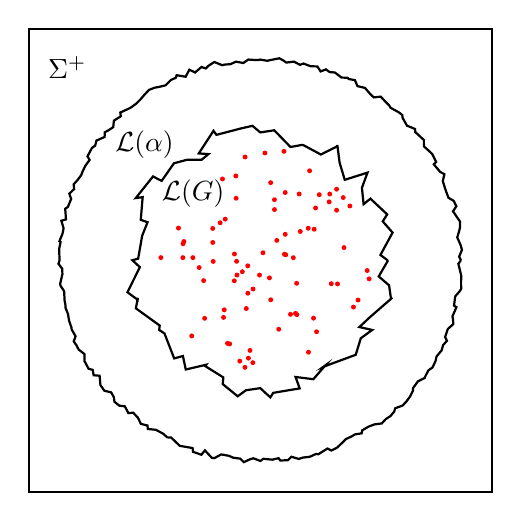
\begin{tikzpicture}[scale=0.98, >=latex]
      % Define center for all sets
      \coordinate (C) at (3,3);

      % Universe: Σ* (The square boundary)
      \draw[thick] (0,0) rectangle (6,6);
      \node at (0.5,5.5) {$\Sigma^+$};

      % Outer curve: L(G) (Syntactically valid - slightly wavy)
      \pgfmathsetseed{12310}
      \begin{scope}[decoration={random steps,segment length=2pt,amplitude=1.02pt}]
        \draw[thick,decorate] (C) circle [radius=2.6];
      \end{scope}
      \node at (1.5,4.5) {$\mathcal{L}(\alpha)$};

      % Middle curve: L(Γ) (Type-safe programs - jagged)
      \begin{scope}[decoration={random steps,segment length=4pt,amplitude=4pt}]
        \draw[thick,decorate] (C) circle [radius=1.65];
      \end{scope}
      \node at (2.13,3.87) {$\mathcal{L}(G)$};

      % Slide 8 Specific: Spray sparse uniform samples strictly inside L(Γ)
      % We use a clip to ensure dots don't bleed over the jagged decoration
      \pgfmathsetseed{20260101}
      \begin{scope}
        \clip (C) circle[radius=1.5];
        \foreach \k in {1,...,80}{
          \pgfmathsetmacro{\rr}{sqrt(rnd)*1.45}
          \pgfmathsetmacro{\tt}{rnd*360}
          \fill[red] ($(C)+(\tt:\rr)$) circle[radius=0.032];
        }
      \end{scope}
    \end{tikzpicture}
  \end{minipage}
  \hfill % This creates the space between the two columns
  % --- RIGHT IMAGE ---
  \begin{minipage}{0.48\textwidth}
    \centering
    \begin{tikzpicture}
      \begin{axis}[
        view={25}{14},
        width=9.2cm,
        height=10cm,
        xmin=-10, xmax=10,
        ymin=-10, ymax=10,
        zmin=0, zmax=8,
        hide axis,
        grid=none,
      ]

        % Paraboloid z = r^2 up to z=8
        \pgfmathsetmacro\R{sqrt(8)}
        \addplot3[
        surf,
        shader=interp,
        opacity=0.3,
        colormap/viridis,
        domain=0:360,
        y domain=0:\R,
        samples=55,
        samples y=25
        ] ({y*cos(x)}, {y*sin(x)}, {y^2});

        % Draw jagged level sets at z = 1,3,5,7
        \pgfmathsetseed{12310}
        \foreach \z [count=\i] in {1,3,5,7}{
          % Inner jagged circle
          \pgfmathsetmacro\rinner{sqrt(\z/0.9)}
          \def\innerpoints{}
          \foreach \sample in {1,...,20}{
            \pgfmathsetmacro\ang{360*\sample/20}
            \pgfmathsetmacro\noise{0.4 * rand}
            \pgfmathsetmacro\x{ (\rinner + \noise) * cos(\ang) }
            \pgfmathsetmacro\y{ (\rinner + \noise) * sin(\ang) }
            \xdef\innerpoints{\innerpoints (\x,\y,\z)}
          }
          \addplot3[black, thick] coordinates {\innerpoints} --cycle;

          % Sample points inside the innermost level set
          \pgfmathsetseed{20260101 + \i}
          \def\dotpoints{}
          \pgfmathsetmacro\numdots{3*\i}
          \foreach \k in {1,...,\numdots}{
            \pgfmathsetmacro\rr{sqrt(rnd)*\rinner*0.9}
            \pgfmathsetmacro\tt{rnd*360}
            \pgfmathsetmacro\x{\rr * cos(\tt)}
            \pgfmathsetmacro\y{\rr * sin(\tt)}
            \xdef\dotpoints{\dotpoints (\x,\y,\z)}
          }
          \addplot3[red, only marks, mark=*, mark size=1] coordinates {\dotpoints};

          % Middle jagged circle
          \pgfmathsetmacro\r{sqrt(\z/0.2)}
          \def\middlepoints{}
          \foreach \sample in {1,...,40}{
            \pgfmathsetmacro\ang{360*\sample/40}
            \pgfmathsetmacro\noise{0.3 * rand}
            \pgfmathsetmacro\x{ (\r + \noise) * cos(\ang) }
            \pgfmathsetmacro\y{ (\r + \noise) * sin(\ang) }
            \xdef\middlepoints{\middlepoints (\x,\y,\z)}
          }
          \addplot3[black, thick] coordinates {\middlepoints} --cycle;

          % Outer bounding square
          \pgfmathsetmacro\h{sqrt(\z / 0.1)}
          \addplot3[black, thick] coordinates { (-\h, -\h, \z) (-\h, \h, \z) };
          \addplot3[black, thick] coordinates { (\h, -\h, \z) (\h, \h, \z) };
          \addplot3[black, thick] coordinates { (-\h, -\h, \z) (\h, -\h, \z) };
          \addplot3[black, thick] coordinates { (-\h, \h, \z) (\h, \h, \z) };
        }

      \end{axis}
      \path (current bounding box.north east) coordinate (plotNE);

      % Labels
      \node[font=\scriptsize, anchor=north west, inner sep=1pt] at ($(plotNE)+(-0.6, -1.3)$) {$\Sigma^{80}$};
      \node[font=\scriptsize, anchor=north west, inner sep=1pt] at ($(plotNE)+(-0.9,-2.9)$)  {$\Sigma^{60}$};
      \node[font=\scriptsize, anchor=north west, inner sep=1pt] at ($(plotNE)+(-1.5,-4.5)$)  {$\Sigma^{40}$};
      \node[font=\scriptsize, anchor=north west, inner sep=1pt] at ($(plotNE)+(-2.2,-5.9)$)  {$\Sigma^{20}$};
    \end{tikzpicture}
  \end{minipage}

  \caption{One can measure the tightness of a sound over-approximation by considering finite models, \vspace{-0.1cm}\[\rho(\alpha, G, m) =  \frac{\sum_{n=1}^m|\mathcal{L}(G) \cap \Sigma^{n}|}{\sum_{n=1}^m|\mathcal{L}(\alpha) \cap \Sigma^{n}|}\text{, which induces an order }\alpha \sqsubset_G^m \alpha' \iff \rho(\alpha', G, m) < \rho(\alpha, G, m). \] where $\rho$ is calculable approximately by Boltzmann sampling or analytically via generating functions.}\label{fig:tightness}
\end{figure}

\bibliographystyle{acl_natbib}
\bibliography{../bib/acmart}
\end{document}